\documentclass{standalone}
\usepackage{tikz}
\usepackage{mathrsfs}
\usetikzlibrary{positioning, shapes.geometric, arrows}
\usepackage[T1]{fontenc}
\renewcommand*\familydefault{\ttdefault} %% Only if the base font of the document is to be typewriter style
\begin{document}
	 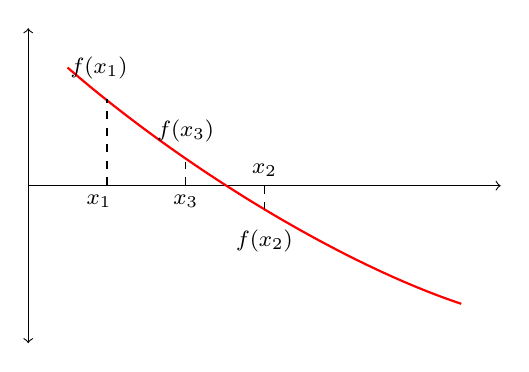
\begin{tikzpicture}[font=\footnotesize]
		\draw[->](0,0) -- (6,0);
		\draw[<->](0,-2) -- (0,2);
		\draw [thick, red] (0.5,1.5) .. controls (2,0.2) and (4,-1) .. (5.5,-1.5);
		\draw[dashed] (1,0) -- (1,1.1);
		\draw (0.9,-0.2) node {$x_{1}$};
		\draw (0.9,1.5) node {$f(x_{1})$}; 
		\draw (3,0.2) node {$x_{2}$};
		\draw [dashed] (3,0) -- (3,-0.3);
		\draw (3,-0.7) node {$f(x_{2})$};\pause
		\draw (2,-0.2) node {$x_{3}$};
		\draw [dashed] (2,0) -- (2,0.3);
		\draw (2,0.7) node {$f(x_{3})$};
	\end{tikzpicture}
\end{document}